\section{Hidden Markov model}

If we may not observe directly the states, we get another Bayesian network named as a Hidden Markov model.
A Hidden Markov model is described by a quintuple $\left\langle S,E,P,A,B \right\rangle$, where: 
\begin{itemize}
    \item $S=\{S_1,\dots,S_N\}$: represents the values for the hidden states.
    \item $E=\{e_1,\dots,e_T\}$: represents the values for the observations. 
    \item $\Pr$: the probability distribution of the initial state.
    \item $A$: the transition probability matrix.
    \item $B$: the emission probability matrix.
\end{itemize}
\begin{example}
    Consider a Markov chain describing weather states with the set of states
    \[\{S_{\text{sunny}},S_{\text{rainy}},S_{\text{snowy}}\}\] 
    The corresponding graph is as follows: 
    \begin{figure}[H]
        \centering
        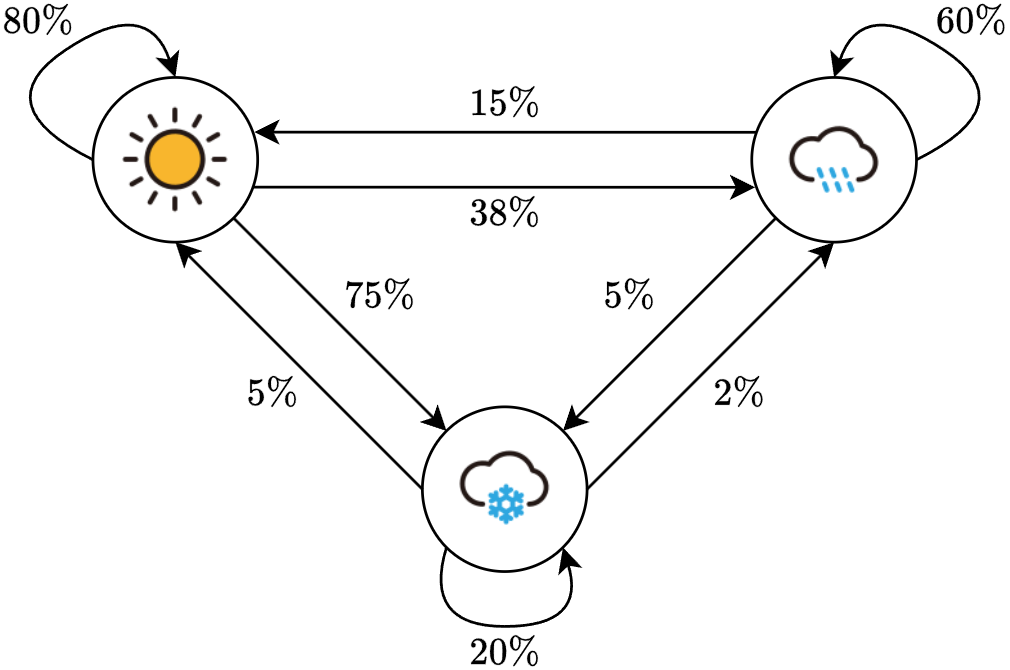
\includegraphics[width=0.4\linewidth]{images/hmm.png}
    \end{figure}
    The corresponding transition matrix is given by:
    \[P=
    \begin{bmatrix}
        0.80 & 0.15 & 0.05 \\
        0.38 & 0.60 & 0.02 \\
        0.75 & 0.05 & 0.20 
    \end{bmatrix}\]
    The initial state distribution is given by $q=\left(\begin{matrix} 0.7 & 0.25 & 0.05 \end{matrix}\right)$, representing a typical day in the considered region.

    Suppose we have the series: sunny, rainy, rainy, rainy, snowy, snowy. 
    The probability of this series is calculated as follows:
    \begin{multline*}
        \Pr(S) = \Pr (S_{\text{sunny}})  \Pr (S_{\text{rainy}}\mid S_{\text{sunny}})  \Pr (S_{\text{rainy}}\mid S_{\text{rainy}})  \Pr (S_{\text{rainy}}\mid S_{\text{rainy}}) \\ \Pr (S_{\text{snowy}}\mid S_{\text{rainy}})  \Pr (S_{\text{snowy}}\mid S_{\text{snowy}}) 
    \end{multline*}
    That is equal to: 
    \[\Pr(S) = 0.7 \cdot 0.15 \cdot 0.6 \cdot 0.6 \cdot 0.02 \cdot 0.2 = 0.0001512\]

    Now, we introduce three observations for each state $\{O_{\text{shorts}},O_{\text{coat}},O_{\text{umbrella}}\}$. 
    In this case, in addition to the transition matrix $A$, we have an observation matrix $B$: 
    \[B= 
    \begin{bmatrix}
        0.60 & 0.30 & 0.10 \\
        0.05 & 0.30 & 0.65 \\
        0.00 & 0.50 & 0.50 
    \end{bmatrix}\]
    Here, states are represented by rows, and observations are represented by columns. 
    The objective is to compute the probability of a series of observations and, if possible, identify the underlying sequence of states.
\end{example}

\paragraph*{Forward probability}
The forward probability represents the joint probability of actual states and observations and is computed as follows:
\[\Pr(X_t=s_i,e_{1:t})=\sum_j A_{ij}B_{je_t}\Pr(X_{t-1}=s_j,e_{1:t-1})\]
This forward probability serves multiple purposes:
\begin{itemize}
    \item It can be utilized to calculate the probability of the observations:
        \[\Pr(e_{1:t})\]
    \item It can be employed for making predictions about the next state:
        \[\Pr(X_{t+1}=s_i\mid e_{1:t})\]
\end{itemize}

\paragraph*{Viterbi algorithm}
From the given observations, it is feasible to compute the most likely hidden state sequence:
\[\argmax\left[\Pr(X_{1:t}\mid e_{1:t})\right]=\argmax\left[\dfrac{\Pr(X_{1:t},e_{1:t})}{\Pr(e_{1:t})}\right]=\argmax\left[\Pr(X_{1:t},e_{1:t})\right]\]
Applying Bayesian network factorization, we obtain:
\[\Pr(X_{1:t},e_{1:t})=\Pr(X_0)\prod_{i=1:t}\Pr(X_i\mid X_{i-1})\Pr(e_i\mid X_i)\]
The solution we seek minimizes:
\[-\log\Pr(X_{1:t},e_{1:t})=-\log\Pr(X_0)+\sum_{i=1:t}\left(-\log\Pr(X_i\mid X_{i-1})-\log\Pr(e_i\mid X_i)\right)\]
To represent this problem graphically, construct a graph with $1 + tN$ nodes: one initial node and $N$ nodes at each time $i$, where the $j$-th node represents $X_i=s_j$.